\chapter{Sound Event Detection}

\section{Snoring Sounds Detection}

People spend almost a third of their life sleeping, thus the sleep quality is very important to people's health. Most of us  have experienced trouble sleeping just sometimes, while for some people sleep problems occur regularly; in former cases a sleep disorder is diagnosed. Among these, one of the most common sleep disorder \cite{sleep-disorders} is the chronic snoring.
Snoring is a noise produced when vibration occurs at several levels of the upper airway. It may be associated with various degrees of upper airway resistance. It is a highly prevalent disorder among the community: it has been confirmed that approximately 30\% of the overall population suffers from chronic snoring almost every night \cite{young1997nasal}.

Sound snoring can have a negative impact on normal physical, mental, social and emotional functioning of the person suffering from it and their bed partner \cite{blumen2012snoring}.  It is also a typical symptom for Obstructive Sleep Apnea (OSA), a chronic sleep disease sharing a frequent occurrence \cite{strollo1996obstructive}. 
OSA is characterised by posterior pharyngeal occlusion for at least ten seconds with apnea/hypopnea and attendant arterial oxyhemoglobin desaturation. If left untreated, this life-threatening sleep disorder may induce high blood pressure, coronary heart disease, pulmonary heart failure and even nocturnal death \cite{banno2007sleep}. In addition, OSA is indicated between the main causes of significant morbidity among children \cite{lumeng2008epidemiology}.

\subsection{Related Works}
\label{ssec:related-works}
Recent studies have found that acoustic signal carries important information about the snore source and obstruction site in the upper airway of OSA patients \cite{pevernagie2010acoustics}. This significant discovery has motivated several researchers to develop acoustic-based approaches that could provide inexpensive, convenient and non-invasive monitoring and screening apparatuses to be combined with traditional diagnostic tools.
The study described in \cite{cavusoglu2007efficient} consists of the identification and segmentation process by using energy and Zero Crossing Rate (ZCR), which were used to determine the boundaries of sound segments. Episodes have been efficiently represented into two-dimensional spectral features by using principal component analysis, and classified as snores or non-snores with Robust Linear Regression (RLR). The system was tested by using the manual annotations of an Ear-Nose-Troth (ENT) specialist as a reference. The accuracy for simple snorers was found to be 97.3\% when the system was trained using only simple snorers' data. It drops to 90.2\% when the training data contain both simple snorers’ and OSA patients' data. In the case of snore episode detection with OSA patients, the accuracy is 86.8\%.
In \cite{qian2015automatic} an automatic detection, segmentation and classification algorithm of Snore Related Signals (SRS) from overnight audio recordings is proposed by combining acoustic signal processing with machine learning techniques.
The specialists have found from OSA patients four classes of SRS, connected to the sound origin mechanism. It is typically defined as the Velum-Oropharyngeal-Tongue-Epiglottis (VOTE) scheme and identifies the tissues in upper airway that are involved in the noise generation.
For classification a k-Nearest Neighbor (k-NN)  model is adopted for its good performance on pattern recognition.  

In the occasion of the Interspeech 2017 ComParE challenge \cite{ComParE2017} and subsequent investigations, different approaches based on Deep Neural Networks (DNNs) have been presented \cite{amiriparian2017snore}, \cite{freitag2017end}, \cite{vesperini2018snore} with the aim to classify isolated snore sound events among the four classes based of the VOTE scheme.

In this work, we propose the application of Convolutional Recurrent Neural Networks (CRNNs) to detect snoring episodes from overnight recordings acquired in real life conditions. The method is a two step process: the acoustic spectral features extraction and the CRNN combined with Gated Recurrent Units (GRU) processing. The algorithm is evaluated by using the Average Precision (AP) score.

Differently from other deep learning approaches \cite{amiriparian2017snore}, \cite{freitag2017end}, \cite{vesperini2018snore}, this choice offers a viable and natural solution for jointly learning the spatio-temporal dependencies of audio sequence for discovering snoring event. Additionally, we deal with the high unbalanced setting which exists in the task of snore detection. The original snore/background ratio in the aforementioned signals has been increased by adding isolated snore events from the Munich-Passau Snore Sound Corpus dataset \cite{ComParE2017}. The reliability of the proposed approach is investigated using the A3-snore dataset, leading to significant improvement in term of Average Precision (AP) with respect to Convolutional Neural Network (up to 9.48\%) and other data augmentation techniques. % (i.e., majority class under sampling 30.15\%, SMOTE \cite{chawla2002smote} 14.23\%).

The outline of this paper is the following. \secref{sec:proposed-approach} describes the acoustic features extraction procedure and the employed DNN architecture. \secref{sec:experiments} are reports the dataset details, the evaluated data augmentation techniques and the experimental set-up. \secref{sec:results} reports the results of the best performing models and \secref{sec:conclusion} concludes this contribution and presents future development ideas.

\section{Proposed Approach}
\label{sec:proposed-approach}

The two step of the proposed approach are detailed in this section, starting from the spectral features extraction and ending with the Convolutional Recurrent Neural Network.

\begin{figure}[t]
	\centering
	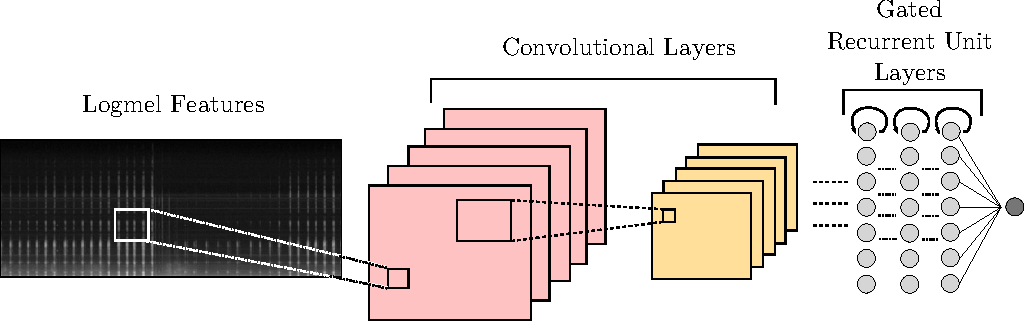
\includegraphics[width=\columnwidth]{img/snore_detection_4.pdf}
	\caption{The proposed approach scheme.}\label{fig:overall}
\end{figure}

\subsection{Features Extraction}
\label{ssec:feat}
The feature extraction stage operates on stereo audio signals sampled at 44.1 kHz. 
Following the results obtained in recent works related to sound event detection \cite{DCASE2017Workshop}, we use the log Mel energy coefficients (Logmel) as an efficient representation of the audio signal. The stereo signal is firstly down-mixed to mono by averaging the two channels. 
The resulting audio signal is split into 30\,ms frames and a frame step of 10\,ms, then the Logmel coefficients are obtained by filtering the power spectrogram of the frame by means of a mel filter-bank, then applying a logarithmic  transformation to each sub-band energy in order to match the human perception of loudness. We used a filter bank with 40 mel scaled channels, obtaining 40 coefficients/frame. 

\subsubsection{Convolutional Recurrent Neural Networks}
\label{ssec:CNN}

CRNNs used in this work are composed of four types of layers: convolutional layers, pooling layers, recurrent layers and detection layer. 

The mathematical operation of convolution has been introduced in artificial neural network layers since 1998 \cite{lecun1998gradient} for image processing. 
Recently CNNs have been often used also in audio tasks, where they exploit one input dimension to keep track of the temporal evolution of a signal \cite{vesperini2018localizing}. In this particular case, the CNNs perform better with filter size small with respect to the input matrix, and this means the temporal context observed in these layers is typically less than two hundred milliseconds.
Each convolutional layer is followed by batch normalization per feature map \cite{ioffe2015batch}, a leaky rectified linear unit activation function (LeakyReLU) and a dropout layer \cite{srivastava2014dropout} with rate equal to $0.3$.
A frequency domain max-pooling layer is then applied to the resulting feature-map, in order to enhance the relevant information from frequency bands without lose the temporal resolution of the Logmels, as proposed in \cite{cakirconvolutional}.
The extracted features over the CNN feature maps are stacked along the frequency axis.
Max-Pooling operation combined with shared weight in convolutional layers provide robustness to frequency shifts in the input features and this is crucial to overcome the problem of intra-class acoustic variability for snore events.

In the recurrent block, the stacked features resulting from the last pooling layer are fed to layers composed of GRUs \cite{chung2014empirical}, where tanh and hard sigmoid activation functions are used for update and reset gates, respectively.
GRU layers control the information flow through a gated unit structure, which depends on the layer input, on the activation at the previous frame and on the reset gate.
%For frame t, the total activation of GRU layer is a linear
%interpolation of previous activation h t−1 and the candidate activation ĥ t as
%%$h t = u t · h t−1 + (1 − u t ) · ĥ tù$ where u t denotes the update gate. 
%Candidate activation ĥ t is a function of h t−1 , the GRU layer’s input x t and the reset gate r t . 
% gRU activation is mainly controlled by reset gate when the GRU layer’s input x t is significantly different than in previous frames. When
%reset gate is closed (r t = 0), the candidate activation does not include any contribution from h t−1 . 
Fast response to the changes in the input and the previous activation information is fundamental for high performance in the proposed algorithm, where the task is to detect a small chunk of consecutive time frames where the target event is present. In addition, a previous work \cite{valenti2017neural} demonstrates improvements provided by recurrent architectures in the sound event detection in real-life audio.

The detection layer is a feed-forward layer of composed of a single neuron with sigmoid activation function, corresponding to the probability the event onset. The layer is time distributed, this means that while computing the output of the classification layer, the same weight and bias values are used over the recurrent layer outputs for each frame.

In a comparative aim, we implemented also a CNN architecture very similar to the CRNN, the only difference being that the recurrent layers of the CRNN are replaced with time distributed feed-forward layers with ReLU activations. In following section, we will refer it as CNN.

%which is an extension of the Adagrad \cite{duchi2011adaptive} algorithm. It was chosen because it is well-suited for dealing with sparse data and its robustness to different choices of model hyperparameters. Furthermore no manual tuning of learning rate is required.
The neural networks training was accomplished by the AdaDelta stochastic gradient based optimisation algorithm \cite{zeiler2012adadelta} for a maximum of 500 epochs on the binary cross entropy loss function. The optimizer hyperparameters were set according to \cite{zeiler2012adadelta} (i.e., initial learning rate $lr=1.0$, $\rho=0.95$, $\epsilon=10^{-6}$). An early stopping strategy, monitoring the validation AP score, was employed in order to reduce the computational burden and avoid overfitting. % Thus if the validation AP does not increase for 20 consecutive epochs, the training is stopped and the last saved model is selected as the final model. 

\section{Experiments}
\label{sec:experiments}
This section details the composition of the dataset used in this work, the data augmentation techniques, the performance metrics and the experimental set-up.

\subsection{Dataset} 
\label{ssec:dataset}
The snore detection algorithm has been evaluated on the A3-Snore dataset. A brief description of the acquisition setup and dataset splitting is provided in the following.

\subsubsection{Acquisition setup:}
In order to capture the overnight audio recordings a ZOOM-H1 Handy Recorder has been used. It is equipped with two unidirectional microphones set at a 90 degree angle relative to one another. The signals are stored in WAV files with a sampling rate of 44.1\ kHz and bit depth equal to 16.
The input gain is automatically set by the recorder to prevent overload and distortion, while the high-pass filter was enabled in order to eliminate pops, wind noise, blowing, and other kinds of low frequency rumble.


\subsubsection{Acquisition environment:}
The acquisition environment consist of a simple bedroom, with two access points (door and window). The recorder is placed near the patient, at same height of the bed and in line with the subject's mouth. During the recordings, the patient is the only one that can occupy the bedroom, in order to avoid contaminations on recorded audio signals. The room dimensions are reported in \figref{fig:room}.
Background sounds include traffic noise, breathing and speech signals, house and animal noises. We acquired some samples measurements of the event-to-background (EBR) ratios considering background noise, snoring events and noise events such as ``car passing by'' or ``dog barfing''. The EBR resulted equal to 6.5 dB and 1.1 dB respectively for noise to background EBR and snore to background EBR. 


\begin{figure}[t]
	\centering
	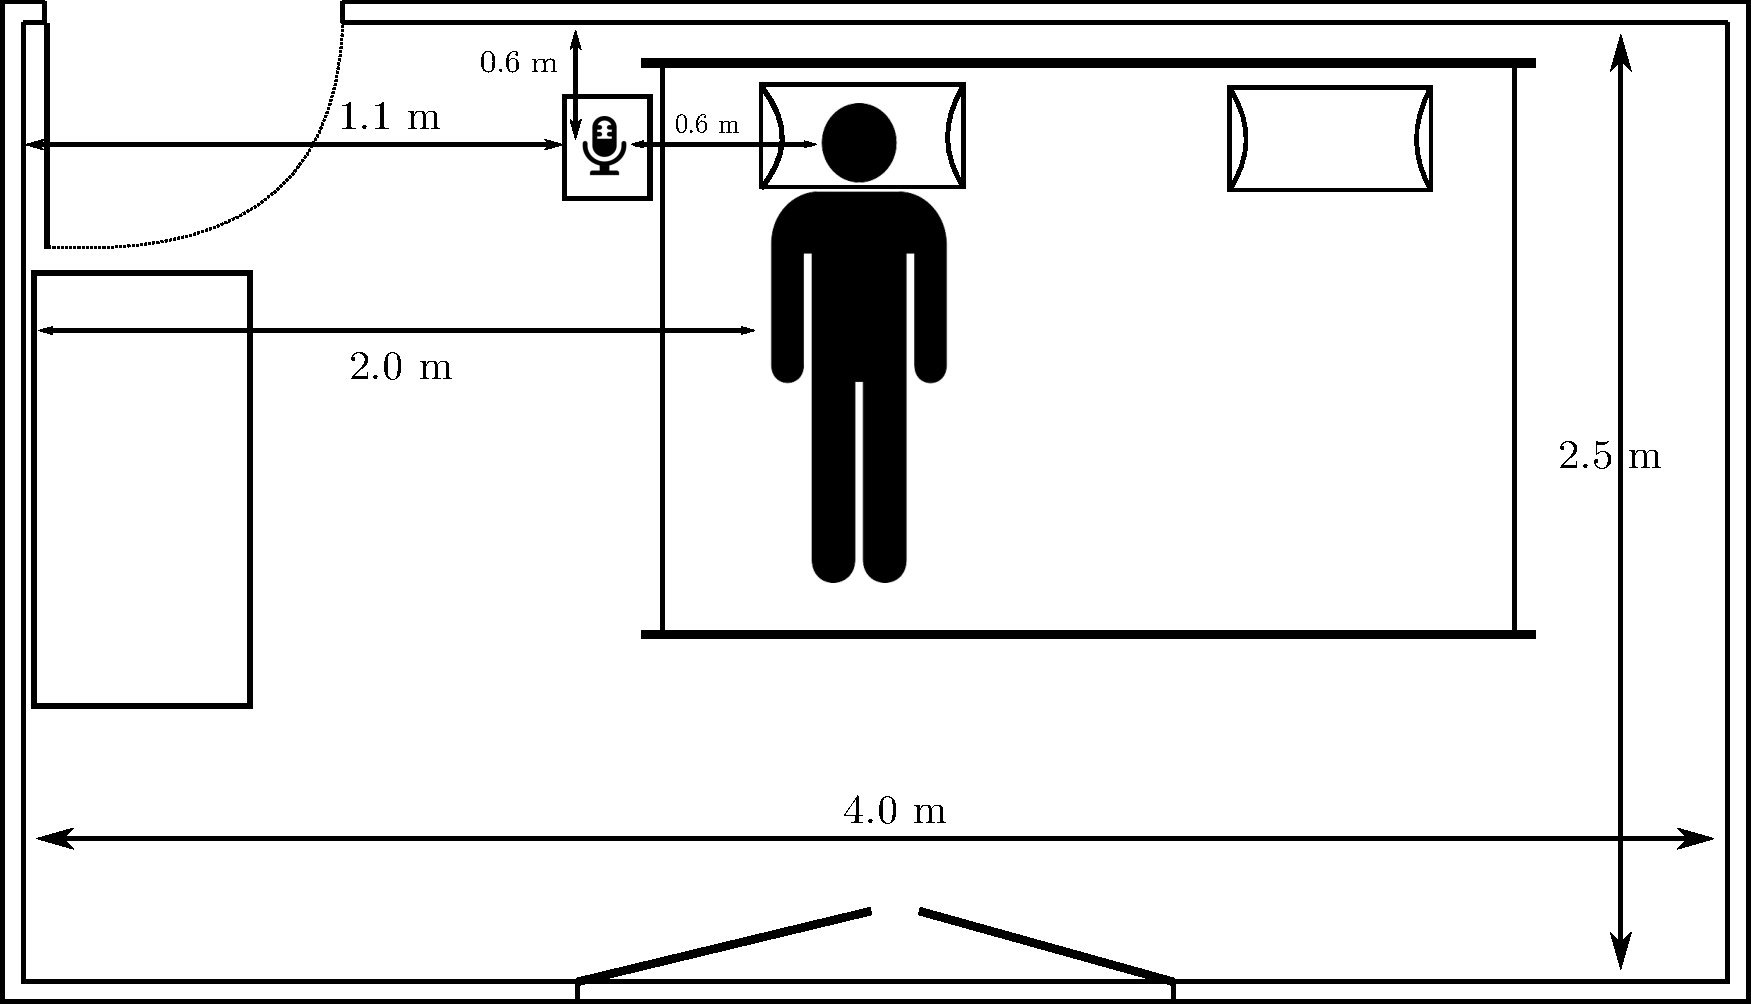
\includegraphics[width=0.8\columnwidth]{img/room.pdf}
	\caption{Plant of the recording room.} 
	\label{fig:room}
\end{figure}


\subsubsection{Dataset splitting:}
The original recordings have been manually labelled, annotating the snore events onset and offset with a resolution of 1 second. The audio sequences have been divided into chunks of 10 minutes, and only those with the highest number of snore events have been used in the experiments. 
The dataset is organized into subjects, which can be respectively used as \emph{training} or \emph{validation} sets in a two fold cross validation strategy (i.e., Leave One Subject Out procedure). The number of events per class in the database is strongly unbalanced as reported in \tableref{a3snore}. Thus, the snore detection task is challenging, due to the high number of noises on the A3-SNORE dataset. 

\begin{table}[ht]
	\centering
	\caption[A3-SNORE dataset]{Difference of recording times for each class, divided by snorers.}
	\begin{tabular}{cccccc}
		\hline
		\multicolumn{6}{c}{\textbf{A3-SNORE dataset}} \\
		\hline
		\# & Gender & Age & Snoring (SN) & Total Duration (Tot) & Ratio (SN/Tot) \\
		\hline
		Snorer 1 & M & 48 & 33m-27s & 3h-12m-0s & 14.5\% \\
		Snorer 2 & M & 55 & 21m-21s & 3h-50m-0s & 11.1\% \\
		\hline
		\multicolumn{3}{l}{Total} &	54m-48s	& 7h-02m-0s	& 12.8\%\\
		\hline    
	\end{tabular}	
	\label{a3snore} 
\end{table}

\subsection{Data Augmentation Techniques}
\label{ssec:data-augmentation}
In this application, what we are really interested is to detect the minority class (e.g. snoring events) rather than the majority class (e.g. background). Thus, we need to adequately train the models in order to obtain a fairly high prediction for the minority class. In order to counteract the dataset unbalancing existing in the task of snoring detection different techniques of data augmentation have been evaluated. 
The literature suggests that it is possible to augment training data in data-space or in feature-space. 
In this work, both data augmentation approach have been evaluated, by using the \emph{Synthetic Minority Over-sampling Technique} (SMOTE) \cite{chawla2002smote} in the feature space, and by generating simulated data with an increased number of snore events. 
The original snore/background ratio in the acquired signals has been increased with these transformations to approximately 30\% \cite{young1997nasal}, maintaining anyway a natural unbalance which is properly of this task.
%TODO: come motivare ratio - ASK LUCA
In the following sub-sections, a brief description of each method is provided.

\subsubsection{Majority Class under sampling:} it is not a properly data augmentation technique but it is a fast and easy way to balance the data. It consists in randomly selecting a subset of data from the training sets in order to modify the ratio of the sample occurrences in two classes.

\subsubsection{SMOTE:} It is an over-sampling approach in which the minority class is over-sampled by creating new synthetic examples. The minority class is over-sampled by taking each minority class sample and introducing synthetic examples along the line segments joining any/all of the \emph{k} minority class nearest neighbors (\emph{k}-NN). Depending upon the amount of required over-sampling, neighbors from the \emph{k}-NNs are randomly chosen. In particular, synthetic samples are generated in the following way: the difference between the feature vector (sample) under consideration and its nearest neighbor is multiplied by a random number between $0$ and $1$, and this is added to the feature vector under consideration. In details, for a sample $x_{i}$:
\begin{equation}
x_{j}^{\text{SMOTE}} = x_{i} + (\tilde{x}_{i,k} - x_{i}) \cdot r(j)
\end{equation}
where $r(j) \in [0,1]$.
This causes the selection of a random point along the line segment between two specific features. This approach effectively forces the decision region of the minority class to become more general. 

\subsubsection{Proposed approach - Generating simulated data:} The simulated training sets have been created starting from the folds described in \secref{ssec:dataset}.
The impulse responses between the snore source and the microphones have been recreated by using the library Pyroomacoustics \cite{Scheibler2018}.
Isolated snore sounds have been taken from the Munich-Passau Snore Sound Corpus (MPSSC) dataset \cite{ComParE2017}. It is composed of 843 snore events which have been extracted and manually screened by medical experts from Drug-Induced Sleep Endoscopy (DISE) examinations of 224 subjects.
The augmented training set has been created by convolving the isolated snore sound events of the MPSSC corpus with the synthetic impulse responses. Than, the obtained signals have been mixed with the original recordings without overlap with the already present events. The artificial added event dynamic was normalized to the maximum value observed in the original signals. The resulting total time of snore signals is 55 minutes for Snorer 1, and 56 minutes and 5 seconds for Snorer 2.

\subsection{Performance Metrics}

The performance of the algorithms has been evaluated in term of AP score, a metric that summarizes the Precision and Recall curve. AP score is calculated as follows:
\begin{equation}
\text{AP} = \sum_n (R_n-R_{n-1})P_n,
\end{equation}
where $R_n$ and $P_n$ are the Recall and Precision for threshold $n$ respectively. Precision and Recall for a generic threshold are calculated as follows:
\begin{equation}
R_n = \frac{TP_n}{TP_n+FN_n}, \quad P_n = \frac{TP_n}{TP_n+FP_n},
\end{equation}
where $TP_n$ is the number of snore frames correctly detected, $FN_n$ is the number of snore frames erroneously detected as background, and $FP_n$ is the number of background frames erroneously detected as snoring.

\subsection{Experimental Setup}
To asses the performance of the models, we explored different hyper-parameter configurations and, for each of these, we repeated the whole experiments training the models both with the original data and  with  data processed with techniques described in \secref{ssec:data-augmentation}. \tableref{CNN-params} shows the hyper-parameter configurations analyzed in our experiments. They regard kernels size, kernel number and GRUs for a total of 120 experiments. In the case of CNN the number of units and layer refers to a Multi Layer Perceptron (MLP) architecture. The experiments were conducted in a 2-fold cross-validation strategy corresponding on a leave one subject out procedure, thus in fold 1 we used Snorer 1 as training set and Snorer 2 as validation set and in fold 2 vice-versa. The models were selected on the performance based on the AP score  averaged on the two folds. 
The algorithm has been implemented in the Python language using Keras \cite{chollet2015keras} as deep learning library. All the experiments were performed on a computer equipped with a 6-core Intel i7, 32\,GB of RAM and two Nvidia Titan X graphic cards. 

\begin{table}[ht]
	\centering
	\caption{Explored network layout parameters.}
	\label{CNN-params}
	\begin{tabular}{|l|r|}
		%		\hline
		%		\multicolumn{2}{|c|}{Network Layout Parameters}            \\ \hline
		\hline
		Convolutional Layers Number & 3                            \\ \hline
		Kernel Number               & 4, 8, 16, 32, 64                 \\ \hline
		Kernel Size                 & $5\times5$, $3\times3$, $2\times2$ \\ \hline
		Pooling Size                & $5\times1$, $4\times1$, $2\times1$ \\ \hline
		\hline
		Recurrent Layers Number     & 2, 3                            \\ \hline
		Dense Layers Number     & 2, 3                            \\ \hline
		Number Of Units             & 4, 8, 16, 32, 64                 \\ \hline
	\end{tabular}
\end{table}


\section{Results}
\label{sec:results}
The performance of the CRNN and CNN architectures using different data augmentation techniques are reported in \figref{fig:results}. In blue are depicted results with CRNN, in green the results of the CNNs. The CRNNs show to be effective for snore event detection yet with the original data, although the dataset imbalance. The best performing model is composed of 3 CNN layers with respectively [64,64,64] filters of size $3\times3$ and two GRU layers of 64 units. This configuration obtains an AP up to 82.05\%, with a difference of +7.79\% with respect to the CNN.

\begin{figure}[t]
	\centering
	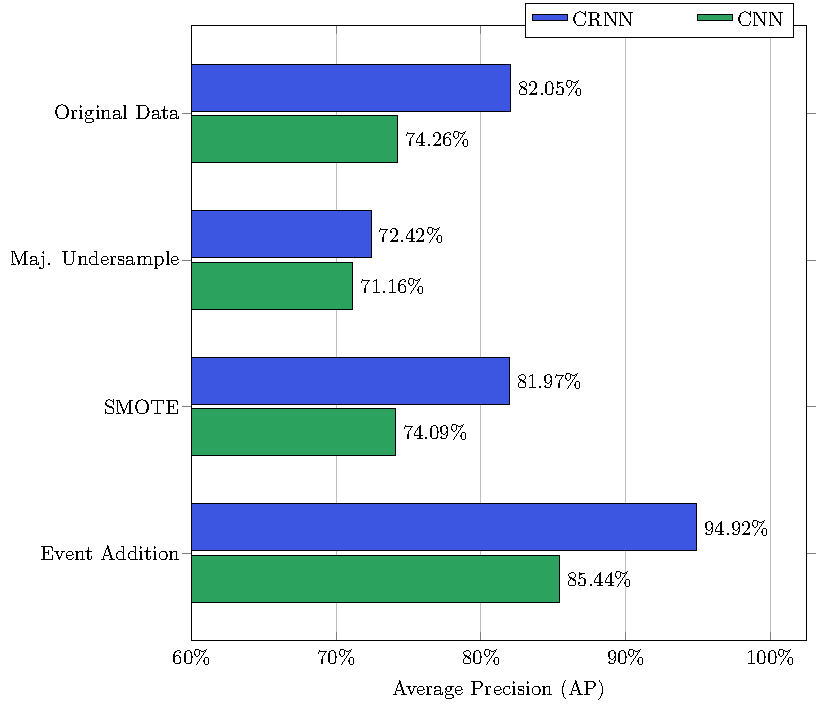
\includegraphics[width=0.7\columnwidth]{img/grafTex/results.pdf}
	\caption{Results with different data augmentation techniques for the best models of the evaluated architectures.} 
	\label{fig:results}
\end{figure}

The majority class under-sampling and the SMOTE techniques obtain worst performance with respect to original recordings. For majority class under sampling this can be motived by the necessity of DNN models of a large amount of data to be trained properly, thus a reduction of data samples cannot benefits to their detection ability. Regarding the SMOTE, the performance reduction is less dramatic (-0.16\% and -0.08\%, respectively, for CNNs and CRNNs) but its employment remains vain. In this case, the motivation can be found on the complexity to generate new samples of audio signals in the feature space which can really improve a DNN perfomance.

The addition of isolated snore samples convolved with the simulated room impulse response has a tangible beneficial effect on the examined models. In fact, with this technique we obtain an AP improvement equal to 11.18\% and 12.87\%, respectively, for the CNN and the CRNN. The latter obtains an AP equal to 94.92\% with an architecture composed of 3 CNN layers with respectively [64,32,32] filters of size $5\times5$ and two GRU layers of 32 units.
This model is composed of 91,553 free-parameters and occupies approximately 1.2 MB, providing to the algorithm a feasible complexity in an application scenario.


\section{Conclusion}
\label{sec:conclusion}
In this paper, a deep learning algorithm based on a CRNN architecture fed with Logmel spectral features extracted from the audio signal has been proposed for snore detection. The A3-Snore dataset has been acquired in real-world conditions, containing overnight recordings of two male subjects and it has been used to assess the performance of the models. The original snore/background ratio has been increased by adding isolated snore events from the Munich-Passau Snore Sound Corpus dataset \cite{ComParE2017}. The reliability of the proposed approach has been investigated with respect to baseline CNN and different data augmentation techniques such as oversampling (i.e., SMOTE) and downsampling. Results show that the presented snore detection methodology is able to better generalize across different users. In particular, the CRNN is able to extract salient information from the spectral features in order to discriminate snore events, while the implemented data augmentation provide additional samples of the minority class (i.e., snore events). These samples contains supplementary information that can be exploited by the CRNN for learning and discriminate snore events.
Future works will be addressed to employ this methodology in a weakly supervised setting.
Specifically, in the real-life applications, the precise annotation of existing events from overnight recordings can be onerous and can be result in sparse labeling. Machine learning models trained in a weakly supervised fashion can help to counteract this problem without losing the state of the art performance.

%%%%%%%%%%%%%%%%%%%%%%%%%%%%%%%%%%%%%%%%%%%%%%%%%%%%%%%%%%%%%%%%%%%%%%%%%%%%%%%%%%%%%%%%%%%%%%%%%%%%%%%%%%%%%%%%%%%%%%%%%%%%%%%%%%

\section{Rare Sound Event Detection}

\section{Introduction}
\label{sec:intro}
Nowadays, one of the most important tasks in the field of computational auditory scene analysis (CASA) is the automatic sound event detection (SED), which can be exploited in various application areas, ranging from acoustic surveillance \cite{clavel2005events,foggia2015reliable} and multimedia event detection \cite{wang2016audio} to smart home devices \cite{krstulovic2018audio,wirn2017-fall, Principi2016a}.
In particular, SED is defined as the task of analysing a continuous audio stream in order to extract a description of the sound events occurring in it. This description is commonly expressed as a label that marks the start, the ending, and the nature of the occurred sound (e.g., children crying, cutlery, glass jingling).

%The 2017 DCASE challenge \cite{DCASE2017Workshop} proposed four different task oriented towards the development of computational scene and event analysis methods by comparing different approaches using common publicly available datasets. 
The ``Detection of rare sound events'' task of the 2017 Detection and Classification of Acoustic Scenes and Events (DCASE) challenge \cite{DCASE2017Workshop} consisted in determining the presence and the precise onset time of three types of sounds, ``baby cry'', ``glass break'' and ``gun shot'' in artificially generated audio sequences. %The background audio material contains recordings from 15 different audio scenes.
The task takes into account real-world issues that introduce additional complexity to the problem, such as the acoustic variability of the sounds belonging to each event class, the presence of environmental noise and its variability, etc. The rules of the challenge allow to know \textit{a priori} the event typology possibly present in the audio sequence under examination, thus it is possible to have a separate binary classifier for each class.

\subsection{Related Works}
In the recent era of the ``Deep Learning'' different approaches to SED have been proposed marking use of the capabilities of deep neural networks (DNNs) to learn the relation between time-frequency features of the raw
audio signal and a target vector representing sound events.
Although the DNNs based systems are more computationally intensive with respect to  widely used statistical modelling methods such as hidden Markov models (HMMs) or Gaussian mixture models (GMMs)  \cite{heittola2010audio, peng2009healthcare}, a comparative study \cite{sigtia2016automatic} has highlighted that they are able to achieve top performance in the sound recognition problem.

A well-fitting example of such performance is given in~\cite{marchi2017deep}, where different DNNs are trained on three datasets recorded in real life environments in order to detect abnormal events or hazardous situations exploiting only the information carried by the acoustic signal. The experimental results show that Deep Recurrent Neural Networks (DRNNs) outperform the probabilistic approaches over the three databases. 
%Another example focuses on employing Convolutional Neural Networks (CNN)  for Voice Activity Detection in multi-room domestic scenarios (mVAD) \cite{vecchiotti2018convolutional}. The CNN-mVAD results to be effective and outperforms the other method with a significant solidity in terms of performance statistics.

In occasion of the DCASE 2017 challenge, many novel systems featuring deep neural networks have been proposed, in particular involving hybrid architectures making use of Convolutional Neural Networks (CNN) and DRNNs. In detail, both the first two classified algorithms make use of mel spectrogram coefficients as spectral representation of the audio signal which is processed by a CNN with 1D filters in the case of the first ranked \cite{limrare} or by a 2D CNN with frequency pooling in the case of the second classified \cite{cakirconvolutional}. The architectures are, then, combined with recurrent layers to process the features obtained by the convolutional blocks.
In \cite{phan2017dnn} the authors propose a hierarchical structure based on CNNs and DNNs trained with multi-task loss functions. Specifically, in the first stage the networks are trained for background noise rejection, using a weighted loss function to penalize the false positive errors. In the second stage the multi-task loss enables the networks to simultaneously perform the event classification task and the onset time estimation. This approach obtained the third place in the final ranking. 
All of the aforementioned systems largely outperform the baseline system based on a Multi Layer Perceptron architecture (MLP) and Logmel energies as features.
%The baseline system \cite{DCASE2017challenge} is based on a Multi Layer Perceptron architecture (MLP) and log mel energies as features. For each audio frame, the input vector is constructed concatenating 5 adjacent log mel vectors for a total of 200 elements. The ANN architecture consists of two dense layers of 50 hidden units each and one output neuron with sigmoid activation, which indicates the activity of the target class.

\section{Proposed Method}
\label{sec:proposed-meth}
The proposed system is a hierarchical algorithm composed of five stages: the acoustic features extraction (\ref{ssec:feat}),  the event detection stage 1 (\ref{ssec:first_stage}) which produces an output at frame-rate and a dedicated smoothing procedure of this signal (\ref{ssec:post_proc_1}).
Then, a refinement of the previous decision stage (\ref{ssec:refinement}) is performed by a 2D CNN which discards possible false positives detected by the stage 1. The final decision procedure (\ref{ssec:final_decision}) annotates the effective onset time of the active event. In Fig.\ref{fig:flow-chart} the phases of the algorithm are depicted. This is an extended and improved method with respect to our contribution to the DCASE 2017 \cite{vesperinihierarchic}.
%\footnote{A copyright-free and preliminary version of this paper has beenpresented at DCASE 2017 workshop, Munich, Germany.}.

\begin{figure}[t]
	\centering
	\vspace{0.2cm}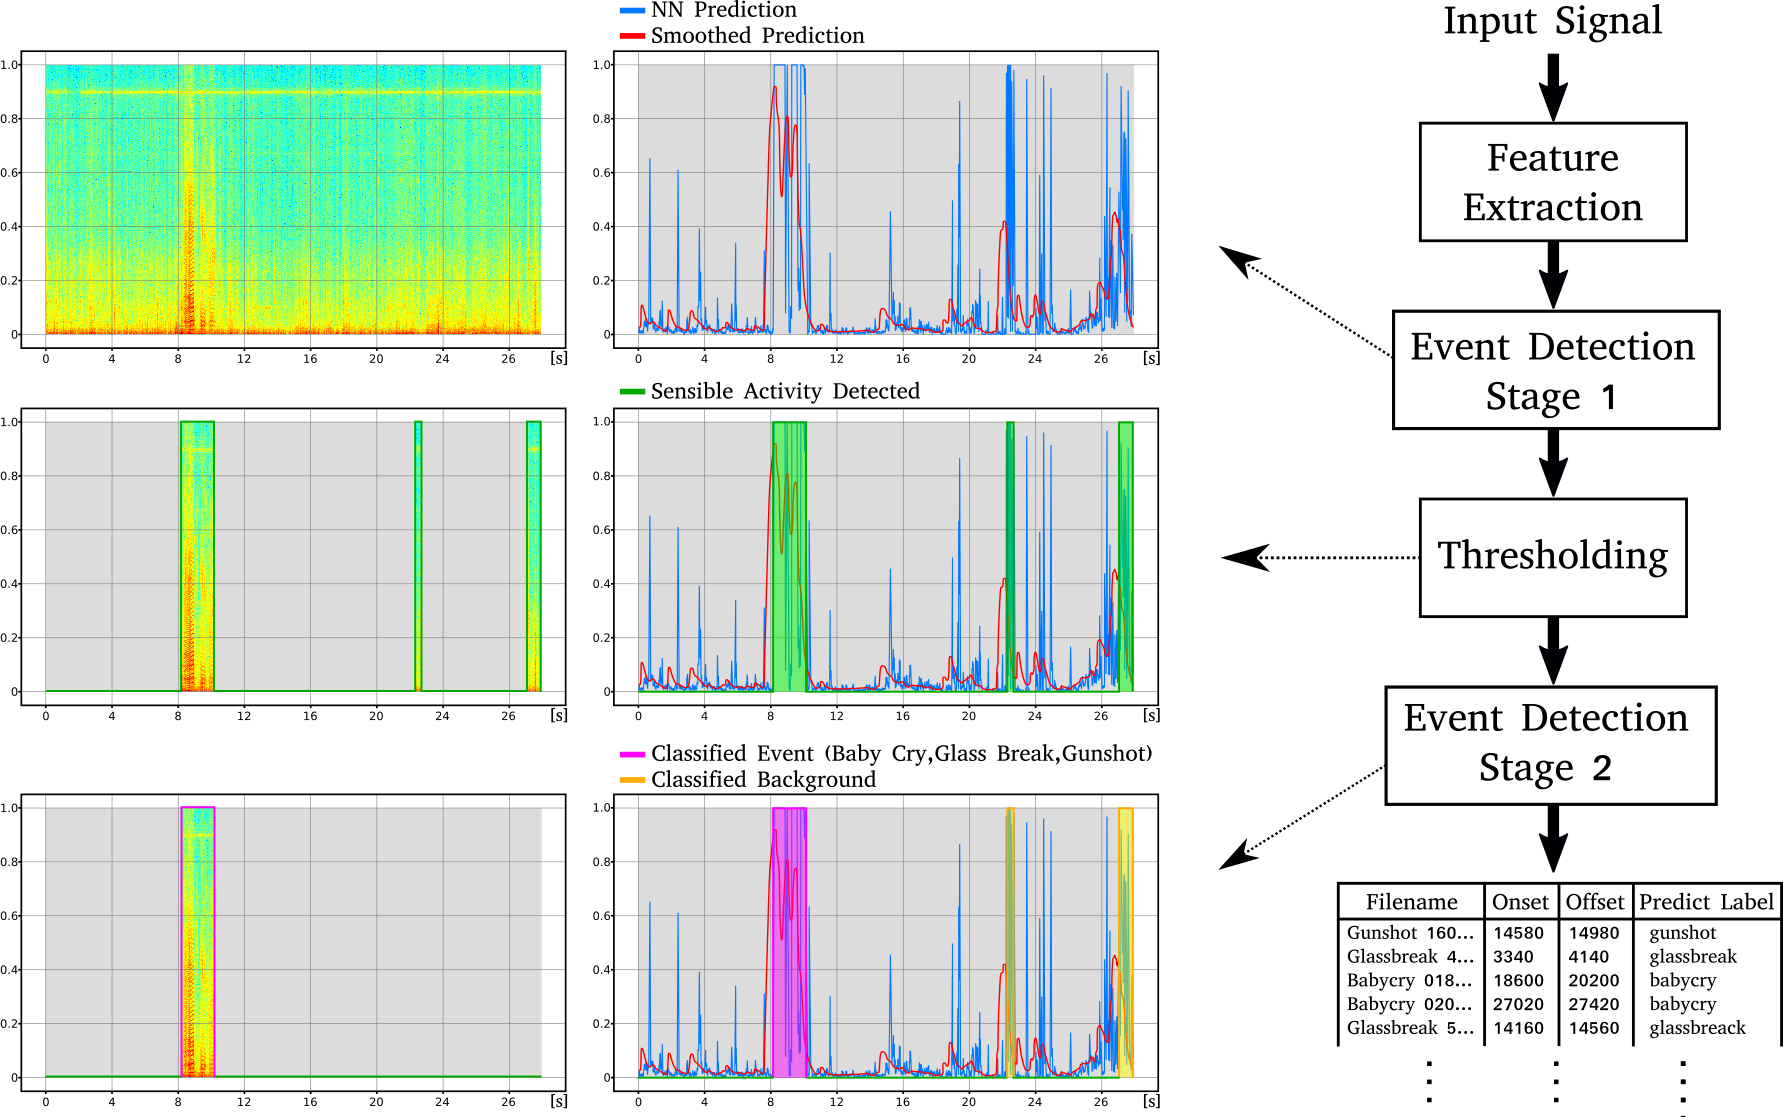
\includegraphics[width=0.97\columnwidth]{Images/approccio_finale_1.png}
	\caption{Flow chart of the proposed method for rare sound event detection. Each event class implements such a scheme. In the first column are shown the spectrograms of the input signal and of the detected events. In the second column the network outputs at each stage of the algorithm.}
	\label{fig:flow-chart}
\end{figure}

\subsection{Features Extraction}
\label{ssec:feat}
The feature extraction stage operates on mono audio signals sampled at 44.1 kHz. 
Following the results obtained at the DCASE2017 challenge by \cite{cakirconvolutional}, we use the log mel energy coefficients (Logmel) as an efficient representation of the audio signal. In addition, we explored the combination of the Logmel with features based on wavelet coefficients and forward prediction errors (WC-LPE) \cite{marchi2014multi}. A brief description of the features extraction procedures is given below.
\subsubsection{Logmel coefficients}
The audio signal is split into frames of 40\,ms and a frame step of 20\,ms, then the Logmel coefficients are obtained by filtering the power spectrogram of the frame by means of a mel filter-bank, then applying a logarithmic  transformation to each sub-band energy in order to match the human perception of loudness. We used a filter bank with 40 mel scaled channels, obtaining 40 coefficients/frame. 

\subsubsection{WC-LPE Feature}
The Wavelet Coefficient (WC) and Linear Prediction Error (LPE) feature set relies on non-stationary signal components and it has been successfully exploited for musical note onset detection \cite{marchi2014multi}. WC-LPE extraction is done by first processing the input signal with a Discrete Wavelet Transform (DWT) dyadic tree. Then, each DWT sub-band is filtered by a linear prediction error filter (LPEF), obtaining Forward Prediction Errors (FPE). All LPEF outputs and DWT sub-bands are resampled to an intermediate sampling rate and rectified. The feature set is, finally, created from the DWT sub-bands, their first order time derivatives, the FPE and their first order time derivatives.

For both feature sets the range values of each coefficient is normalized independently according to the mean and the standard deviation computed on the training sets of the neural networks.

\subsection{Event Detection Stage 1}
\label{ssec:first_stage}
The Event detection (ED) stage 1 has the goal to discard frames containing only background sounds, reducing as much as possible the false negative decisions.
We evaluated two DNN architectures as binary classifiers: the MLP and the CNN with 2D kernels and frequency pooling. In both cases, the output layer is formed by two units with the \textit{softmax} non-linear function. Thus, the networks outputs represent the probabilities that an input feature vector $\mathbf{x}[t]$ at the frame index $t$ belongs to the background or the event class. In our analysis, we evaluated as network input the Logmel coefficients and the combination of the latter with the WC-LPE features.

\subsubsection{Multi Layer Perceptron Neural Network}
The artificial neuron is the main element of the MLP. It consists of an activation function applied to the sum of the weighted inputs \cite{Rumelhart86-LRB}. Neurons are then arranged in layers, with feed-forward connections from one layer to the next. The supervised learning of the network makes use of the stochastic gradient descent with error back-propagation algorithm. The network is designed to consider a temporal context  $C$, thus the network input  feature vector  $\hat{\mathbf{x}}[t]$ is obtained concatenating $\mathbf{x}[t]$ with the previous $\mathbf{x}[t - c]$, with $c = 1, \dots, C$. 
% obtaining:
%\begin{equation}
%\mathbf{x}[t] =  \{\mathbf{x}[t - c],\ldots,\mathbf{x}[t-1],\mathbf{x}[t]\},
%\end{equation}
%with $c = 1, \dots, C$. 
During the training procedure, additive zero-centered Gaussian noise with $\sigma=0.1$ was applied to $\hat{\mathbf{x}}[t]$ as a form of data augmentation, improving the generalization capabilities of the DNN and avoiding overfitting \cite{marchi2017deep}.

%Figure \ref{fig:MLP-train} shows the flow chart of the complete procedure for the MLP-based event detection stage configuration.
%\begin{figure}[t]
%	\centering
%	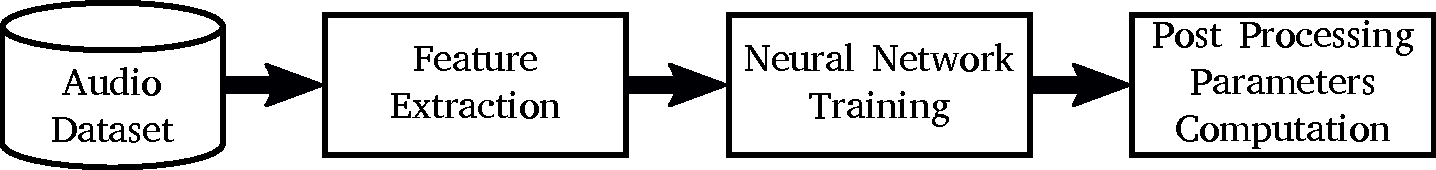
\includegraphics[width=\columnwidth]{Images/training_first_stage.pdf}
%	\caption{Set-up procedure of the MLP-based event detection stage.}
%	\label{fig:MLP-train}
%\end{figure}

\subsubsection{Convolutional Neural Network}
\label{ssec:CNN}
%lavora su base chunk 20 frame: organizzazione input (chunk da 20 non overlappati) e label 
%descrizione di come lavorano i kernel per efatizzare la multiresolution approach
%cleassificazione chunk ovellappati (chunk size -1 )

CNNs are feed-forward neural networks \cite{Yann-cnn-1998} composed of three types of layers: convolutional layers, pooling layers and densely connected layers of neurons. The convolutional layers perform the mathematical operation of convolution between a multi-dimensional input and  kernels of fixed size. The kernels are generally smaller compared to the input, allowing CNNs to process large inputs with a modest number of parameters to learn. CNNs are often used in audio tasks, where they exploit one input dimension to keep track of the temporal evolution of a signal \cite{thomas2014analyzing}.
In our case the convolutional layer input is a matrix $\mathbf{X} \in \mathbb{R}^{F \times T}$, where $F$ and $T$ represent respectively and the number of Logmel channels and the number of frames of the acoustic signal.
When we combine the two aforementioned feature sets, we process them with two separate sets of convolutional layers, gathering two feature maps that are concatenated along the feature axis. Before concatenation, batch normalization \cite{ioffe2015batch} is applied to each feature map and a leaky rectified linear unit activation function (LeakyReLU) with $\alpha=0.3$, followed by a feature domain max-pooling layer.
Finally, fully connected layers are stacked, applying the same weights and biases to each frame element. The output layer for each of the binary classifier neural networks has two neurons corresponding to the probability of the background or the event onset. We can discard, thus, one of the two neurons without loss of information, and we will consider the output of the neuron corresponding to the event activation $u[t] = y_{t,2}$, as the output of the network at frame $t$.

%which is an extension of the Adagrad \cite{duchi2011adaptive} algorithm. It was chosen because it is well-suited for dealing with sparse data and its robustness to different choices of model hyperparameters. Furthermore no manual tuning of learning rate is required.
The neural networks training was accomplished by the AdaDelta stochastic gradient-based optimisation algorithm \cite{zeiler2012adadelta} for a maximum of 500 epochs on the binary cross entropy loss function. The optimizer hyperparameters were set according to \cite{zeiler2012adadelta} (i.e., initial learning rate $lr=1.0$, $\rho=0.95$, $\epsilon=10^{-6}$). An early stopping strategy monitoring the validation loss was employed in order to reduce the computational burden. Thus if the validation loss does not decrease for 20 consecutive epochs, the training is stopped and the last saved model is selected as the final model. In addition, dropout is used as regularization technique \cite{srivastava2014dropout} with rate $0.5$. 

\subsection{Post Processing}
\label{ssec:post_proc_1}
In the post processing stage, each network output is convolved with an exponential decay window of length $M$ defined as:
\begin{equation}
\mathbf{w}[t]= e^{\frac{−t}{\tau}} \quad \text{with}  \, \tau =  \frac{-(M-1)}{log_e(0.01)}
\end{equation}
%\begin{equation}
%\tilde{ \mathbf{u}}[t] = \mathbf{u}[t] \ast \mathbf{w}[t]
%\end{equation}
The result is processed with a sliding median filter with local window-size $k$. Finally, a decision threshold $\theta$ is applied.

\subsection{Event Detection Stage 2}
\label{ssec:refinement}
The aim of the event detection stage 2 is to eliminate false positives, by removing the events wrongly detected at the previous stage. This is done by feeding a binary-classifier CNN with chunks of features in correspondence to the detected events (colored region in the bottom right spectrogram of Figure \ref{fig:flow-chart}). At this stage only Logmel coefficients are used as input features, in order to reduce the computational burden of the model. Non-overlapping feature matrices $\mathbf{X}$ of size $F\times20$ are used during training, while 95\%-overlapping feature matrices are employed during testing (1-frame shift).
A chunk size of 20 corresponds to 0.4 seconds of audio, i.e. half the minimum possible length of the occurring events, leading to an analysis of the audio event at different time and frequency resolutions with respect to previous stages. The ED Stage 2 NN is trained for 100 epochs on the binary cross entropy loss function with the AdaDelta gradient descent algorithm. %In the second stage we employ only log mel coefficients as network input.


\subsection{Final Decision}
\label{ssec:final_decision}
For each audio sequence, we perform a classification on contiguous blocks of frames detected as event by the ED stage 1. Among contiguous frame chunks classified as ``event'' by the CNN, the first frame with highest network output is indicated as event onset.

\section{Dataset}
The DCASE2017 challenge dataset \cite{DCASE2017challenge} has been used to develop and evaluate the algorithm.  The dataset consists of 30-second long sequences of background acoustic scenes recorded in different public or domestic spaces (park, home, street, cafe, train etc.) \cite{mesaros2016tut}, some of which have been added with isolated recordings from at most one of the three different target sound event classes: baby crying, glass breaking and gun shot. 
%The presence probability of a sound event in each mixed sequence is 0.99 for both the training and the validation sets, while the challenge default was 0.5. 
The presence probability of a sound event in each mixed sequence of the original Development set was 0.5, thus we kept only sequences containing a sound event of the original training set and we generated additional mixtures assigned to the training and the validation sets.
For the development set a total number of sequences respectively equal to 2750 for training, 300 for validation and 1496 for test have been employed.
This change increases the percentage of the frames including a target event in the training data, which helps to ease the problem of data imbalance. In addition, due to the fast decay of the ``gun shot'' sound, we generated more sequences containing this event class compared to the others, in order to maintain approximately the same percentage between frames containing event samples and backgrounds.

In the evaluation set, the training and test sequences of the development set are combined into a single training set,  while the validation set is the same used in the Development dataset. The system is evaluated against an ``unseen'' set of 1500 samples (500 for each target class) with a sound event presence probability for each class equal to 0.5.


\section{Experimental Set-Up}
\label{sec:experiment}
According to the DCASE 2017 guidelines, the performance of the proposed algorithm has been assessed by using the development dataset for training and validation of the system. Furthermore, a blind test on the provided evaluation dataset has been performed.
The performance metric of the DCASE 2017 challenge is the event-based error rate (ER) calculated using onset-only condition with a collar of 500 ms. Detailed information on metrics calculation are available in \cite{Mesaros2016_MDPI}. The algorithm has been implemented in the Python language using Keras \cite{chollet2015keras} as deep learning library. All the experiments were performed on a computer equipped with a 6-core Intel i7, 32\,GB of RAM and two Nvidia Titan X graphic cards.


\subsection{First Event Detection Stage}
\label{sec:results}


\begin{table}[b]
	\caption{Hyper-parameters optimized in the random-search phase for the MLP ED stage 1, and their range.}\label{tbl:hyper-params-mlp}
	\centering
	\footnotesize
	\begin{tabular} {|c | c | c|}
		\hline
		Parameter & Range & Distribution\\  
		\hline
		\hline                                     
		MLP layers Nr.  & [2 - 7]& uniform \\
		\hline                                     
		MLP layers dim. & [20 - 4048]& log-unifom \\
		\hline                                     
		MLP Context & [1 - 7] & uniform\\
		\hline
		Activation & [tanh - relu] & uniform\\
		\hline
	\end{tabular}
\end{table}
%%

\begin{table*}[t]	
	\caption{Results in terms of ER score for all the evaluated combination of proposed ANNs and features used in Event Detection Stage 1.}
	\centering
	\footnotesize
	\begin{tabular}{l|c|c|c|c|c|c|c|c|}
		\cline{2-9}
		& \multicolumn{4}{c|}{\textbf{Development Dataset}}          & \multicolumn{4}{c|}{\textbf{Evaluation Dataset}}                 \\ \hline
		\multicolumn{1}{|l|}{Features}         & Babycry & Glassbreak & Gunshot & \textbf{Average} & Babycry & Glassbreak & Gunshot & \textbf{Average} \\ \hline
		\multicolumn{9}{|c|}{\textbf{MLP ED Stage 1 }}                                                                                                          \\ \hline
		\multicolumn{1}{|l|}{Logmel}         & 0.19    & 0.12       & 0.16    & \textbf{0.16}    & 0.64    & 0.54       & 0.58    & 0.59             \\ \hline
		\multicolumn{1}{|l|}{Logmel + WC-LPE} & 0.23    & 0.10       & 0.19    & 0.17             & 0.76   & 0.55       & 0.55    & 0.62             \\ \hline
		\multicolumn{9}{|c|}{\textbf{CNN ED Stage 1}}                                                                                                          \\ \hline
		\multicolumn{1}{|l|}{Logmel}         & 0.23    & 0.13       & 0.18    & 0.18             & 0.48    & 0.23       & 0.44    & 0.38             \\ \hline
		\multicolumn{1}{|l|}{\textbf{Logmel + WC-LPE}} & 0.25    & 0.09       & 0.16    & 0.17             & 0.46    & 0.10       & 0.36    & \textbf{0.31}    \\ \hline
		\hline
		\multicolumn{9}{|c|}{\textbf{MLP ED Stage 1 + CNN ED Stage 2}}                                                                                       \\ \hline
		\multicolumn{1}{|l|}{Logmel}         & 0.14    & 0.08       & 0.16    & \textbf{0.13}    & 0.31    & 0.25       & 0.44    & 0.33             \\ \hline
		\multicolumn{1}{|l|}{Logmel + WC-LPE} & 0.20    & 0.09       & 0.19    & 0.16             & 0.37    & 0.27       & 0.40    & 0.35             \\ \hline
		\multicolumn{9}{|c|}{\textbf{CNN ED Stage 1 + CNN ED Stage 2}}                                                                                        \\ \hline
		\multicolumn{1}{|l|}{Logmel}         & 0.19    & 0.10       & 0.16    & 0.15             & 0.31    & 0.17       & 0.39    & 0.29             \\ \hline
		\multicolumn{1}{|l|}{\textbf{Logmel + WC-LPE}} & 0.18    & 0.08       & 0.17    & 0.14             & 0.25    & 0.10       & 0.31    & \textbf{0.22}    \\ \hline
	\end{tabular}
	\label{tab:results}
\end{table*}

%
To assess the performance of the MLP employed in the event detection stage 1 we resorted to a random search strategy \cite{bergstra2012random}.
Table \ref{tbl:hyper-params-mlp} shows the parameters explored in the random search, as well as the prior distribution and ranges. We evaluated 300 sets of layout parameters (100 for each event class) repeated for the two input features combination.

Regarding the CNNs, we explored the hyper-parameters space by means of a grid search for a total of 75 experiments (25 for each event class) covering the number of convolutional filters per layer $\{16,32,64\}$, the kernels shape $\{3 \times 3, 5 \times 5\}$, the number of MLP layers $\{1,2,3\}$ and their respective number of units $\{16,32,64,128\}$. The feature
max-pool sizes after each convolutional layer were $\{5,4,2\}$ for all the explored layouts. Also in this case the experiments were repeated for both the input features combination.

A successive grid search was performed for each network configuration evaluated, in order to find the post-processing parameters that yielded the minimum error rate. Investigated parameters in the grid search were: exponential window length $w$ in the range $\{10,20,\dots,90\}$, median filter kernel $k$ in the range $\{9,11,\dots,31\}$ and threshold $\theta$ in the range $\{0,0.05,\dots,0.5\}$. 

Once the best models on the Development dataset were found, a fine tuning of the post processing parameters was done during the validation stage, in order to assess the performance of the whole system. In fact, the hierarchical architecture of the algorithm allows to set a lower threshold in the first decision stage in order to reduce the deletions at the expenses of some insertions. These will be removed by the ED stage 2. 

%The respective ranges are reported in Table \ref{tbl:post-proc-params-mlp}. 
%\begin{table}[h]
%	\caption{Post processing parameters optimized in grid search phase, and their ranges.}
%	\label{tbl:post-proc-params-mlp}
%	\centering
%	\footnotesize
%	\begin{tabular} {|l | c | c |}
%		\hline
%		Parameter     & Range  & Step\\  
%		\hline
%		\hline                                     
%		Threshold $\theta$ & [0-0.7] & 0.01\\
%		\hline                                     
%		Window length $M$ & [10-90] & 10 \\
%		\hline
%		Median filter window $k$ & [9-13] & 2\\
%		\hline                                       
%	\end{tabular}
%\end{table}


%\begin{itemize}
%	\item \textbf{Baby cry:} the input layer accepted 156 values for each frame index, corresponding to a context size $C=3$, the hidden layers were three dense layers respectively of size $[2487-898-40]$, to whom the $ReLU$ activation function is applied. The network was trained with the whole 2750 training sequences, then was evaluated with $\theta=0.2$, $w=50$, $k=29$ as post processing parameters.
%	
%	\item \textbf{Glassbreak:} the input layer accepted 52 values for each frame index, corresponding to a context size $C=1$, the hidden layers were three dense layers respectively of size $[3634-1126-95]$, to whom the $ReLU$ activation function is applied. The network was trained with the whole 2750 training sequences, then was evaluated with $\theta=0.28$, $w=50$, $k=29$ as post processing parameters.
%	
%	\item \textbf{Gunshot:} the input layer accepted 52 values for each frame index, corresponding to a context size $C=1$, the hidden layers were four dense layers respectively of size $[3031-493-108-45]$, to whom the $ReLU$ activation function is applied. We noticed that in this case the network achieve better performance if it was trained specifically with the 1250 sequences containing only the ``gunshot'' event, then was evaluated with $\theta=0.23$, $w=40$, $k=23$ as post processing parameters.
%\end{itemize}

\subsection{Refinement Stage}

%Per trainare la cnn abbiamo data in ingresso alla prima rete delle sequenze audio di solo bck. Gli eventi selezionati da questa rete rappresentano il materiale di training
%della classe bck per la cnn. Per le altre classi di eventi abbbiamo preso le porzioni di soli eventi mixed to bck relativi alle mixture fornite dal dcase e gli isolated events.
%
%Abbiamo generato una stratified validation split del dataset appena descritto. 
%Abbiamo effetuato una valutazione della cnn subase evento con la fmeasure.
%Finally, sul validati

\subsubsection{Training set for CNN based ED Stage 2 }
To compose the dataset for training and evaluation of the CNNs dedicated to each target audio event we proceeded as follows: the samples of each event class were selected between the audio sections respectively labelled as ``baby cry'', ``glass break'' and ``gun shot'' from the mixtures of the DCASE 2017 development dataset, in addition with the isolated events source signals. To obtain the background samples, we processed with the first stage of our algorithm sequences from the same dataset which do not contain events. 
Thus, the frames detected as event in this case represent the ``false positive'' or ``insertions'' of the stage 1. 
%We used those frames as background samples in the CNN training phase to improve its refinement in the event detection process and balancing the dataset. 
We used those frames as background samples in the CNN training phase to improve its event classification abilities and balancing the dataset. 


To design the best refinement CNN model for our purposes, we generated a shuffle stratified validation split from the dataset composed as described above. We left out the 30\% of the samples as validation set for the CNN model and we selected the layout parameters of the neural network based on the F-measure score obtained on this data sub-set. 
The best performing model was the same for all the target audio events and was composed as follows: three convolutional layers with $\{32,32,32\}$ filters, respectively, of size $5\times5$. The convolutional layers were followed by a feature max pooling layer with kernels of size $\{5,4,2\}$, respectively. Three dense layers composed of 32 neurons with $tanh$ activation functions were applied before the network output layer, for a total number of network parameters equal to 35K. 

%Descrizione con img della fase di valutazione
%Scelta th 0.20 invece c he 0.25: per favorile meno deletion a discapito delle insertion. La cnn pensa a eliminare le insertion classificandole come bck

%\textcolor{red}{A complete overview of the parameters of the best performing system are reported in Table YY}. 
%It is necessary to remark that in this challenge task the event target class (not its presence or absence) was a prior knowledge, thus in evaluation phase the illustrated procedure is applicable independently to different sequences each potentially containing the respective target event. The final score is then computed overall.
%\textcolor{red}{In table YY are reported the parameters used in each of the four submission that we performed}. 

\section{Results}
Results reported in Table \ref{tab:results} are obtained as follows: we selected the models with lowest ER for each combination of DNN architecture and input features operating in the ED stage 1 and we evaluated the systems separately for each target class before the ED stage 2 on the Evaluation set, keeping ED stage 1 post processing parameters fixed. Then, with the same settings we obtained the performance of the whole system both on Development and Evaluation datasets. The architecture composed of a first stage with 2D CNN fed by Logmel and WC-LPE features resulted the best performing on the Evaluation dataset, obtaining an average ER equal to 0.17.
% cnn dedicated to ``babycry'' and ``gunshot'' events have approximately the same number of free parameters and obtain respectively an ER equal to 0.25 and 0.16. The ``glassbreak'' architecture 
Details of these architectures are reported in Table \ref{tab:CNN_details}.
%\begin{table}[]
%	\centering
%	\footnotesize
%	\caption{My caption}
%	\label{my-label}
%	\begin{tabular}{@{}l|c|c|c@{}}
%		\toprule
%		Hyper-parameters & Babycry                                 & Glassbreak                  & Gunshot           \\ 
%		\midrule
%		Conv. Kernels    & 5$\times$5, 3$\times$3, 3$\times$3 					 & 3$\times$3, 3$\times$3, 3$\times$3 					& 3$\times$3, 3$\times$3, 3$\times$3 \\
%		Kernel shape     & 32, 16, 16                         & 64, 64, 64                         & 32, 16, 16   \\
%		MLP Layers size  & 32, 32                            & 128, 128                             & 32, 32      \\ \midrule
%		\# Parameters    & 18K                                  & 185K                                  & 17K            \\ \bottomrule
%	\end{tabular}
%\end{table}

\begin{table}[b]
	\centering	
	\footnotesize
	\caption{Details of models for CNN based ED stage 1 with the lowest ER on Development set. All of them use a combination of log mel energies and WC-LPE as input features.}
	\label{tab:CNN_details}
	\resizebox{\columnwidth}{!}{
		\begin{tabular}{|l|c|c|c|}
			\hline
			Hyper-parameters & Babycry                            & Glassbreak                         & Gunshot                            \\ \hline
			Conv. Kernels    & 5$\times$5, 3$\times$3, 3$\times$3 & 3$\times$3, 3$\times$3, 3$\times$3 & 3$\times$3, 3$\times$3, 3$\times$3 \\
			Kernel shape     & 32, 16, 16                         & 64, 64, 64                         & 32, 16, 16                         \\
			MLP Layers size  & 32, 32                             & 128, 128                           & 32, 32                             \\ \hline
			\# Parameters    & 18K                            & 185K                            & 17K                            \\ \hline
		\end{tabular}
	}
\end{table}
The experimental results show how this combination improves generalization properties of the algorithm. In fact, the MLP based stage 1 with only Logmel features obtains the best overall ER equal to 0.13 on the Development dataset, but the performance decreases significantly on the Evaluation set. In addition, the number of free parameters of the best performing MLP models was always an order of magnitude greater w.r.t. the CNN models. Regarding the stage 2, its beneficial effect is supported especially with the Evaluation dataset: in this case, the improvement in terms of ER given by the joint detection procedure is evident and it gives additional robustness to the system in terms of generalization.

In Table \ref{tab:params} the overall results between best ranked systems of the DCASE 2017 Challenge are compared. It can be observed that the best two scores have been obtained with ensemble methods, involving the additional computational cost of running several architectures in parallel, while the table reports the number of parameters per architecture. Although the proposed system does not outperform the first two methods, the average number of network parameters is significantly lower. This provides greater scalability in real-world applications.

\begin{table}[t]
	\centering
	\footnotesize
	\caption{Comparison between the obtained ER scores and the number of parameters with the first three ranked approaches at the DCASE2017 Challenge.}
	\label{tab:params}
	\begin{tabular}{|l|c|c|}
		\hline
		Approach        & Evaluation ER & \# Parameters \\ \hline
		Lim et al. \cite{limrare}      & \textbf{0.13}                               & 6200K          \\ 
		Cakir et al.  \cite{cakirconvolutional}   & 0.17                               & 756K          \\ 
		Proposed system & 0.22                               & \textbf{108K}         \\ 
		Phan et al. \cite{phan2017dnn}   & 0.27                               & 2100K          \\ \hline
	\end{tabular}
\end{table}


\section{Conclusion}
In this paper, a framework that makes use of hierarchical CNN classifiers fed with Logmel and WC-LPE features has been proposed for rare SED, providing significantly improved performance over the baseline system for every target sound event class in DCASE 2017 challenge dataset. The system also provides a significant reduction of the network parameters w.r.t. other competitive algorithms.  
The multi-scaled approach inherent to the two different CNN architectures results to be effective. 

For future work, strategies to customize the loss function embedding the evaluation metric into the training procedure can be considered. Specifically, this task is particularly affected by the dataset unbalancing: to counteract this problem an alternative to the data augmentation is to design tailored loss functions which enhance the detection of the rare events. 
%In addition, recurrent architectures can be combined with the CNNs in order to exploit the information carried by the temporal evolution of the acoustic signal.% and to evaluate the amount of the supplementary computational burden.

%%%%%%%%%%%%%%%%%%%%%%%%%%%%%%%%%%%%%%%%%%%%%%%%%%%%%%%%%%%%%%%%%%%%%%%%%%%%%%%%%%%%%%%%%%%%%%%%%%%%%%%%%%%%%%%%%%%%%%%%%%%%%%%%%%
\section{Sound Event Detection in Real Life Audio}

\section{Introduction}
\label{sec:intro}


Automatic sound event detection (SED), also known as acoustic event detection, is nowadays considered as one of the most important topics in the field of computational auditory scene analysis (CASA). Thanks to works like Bregman's ``Auditory Scene Analysis: The Perceptual Organization of Sound''~\cite{bregman1994auditory}, we can trace back the birth of this field to 1994, when the field of auditory scene analysis (ASA) was introduced in order to model humans' sound perception. Following this work, many other contributions were written aiming to describe how artificial systems can be designed in order to perceive sounds similarly to as humans do; most of these works will be later collected in Divenyi's book~\cite{divenyi2004speech} in 2004.

SED is defined as the task of analysing a continuous audio signal in order to extract a description of the sound events occurring in the audio stream. This description is commonly expressed as a label that marks the start, the ending, and the nature of the occurred sound (\emph{e.g.,}\ children crying, cutlery, glass jingling). In particular, in multi-label SED it is assumed that more than one event can be active (and should be detected) at a time, therefore foreseeing the overlapping of two or more of these labels. This problem is addressable as a ``mixture problem'' and it is usually not trivial to solve mainly due to the superimposition of different event energies in the audio spectra.

Labels extracted with a SED system usually allow us to achieve a better insight of the considered acoustic scenario, for example they can be used as mid-level representation useful for other CASA research areas. In~\cite{chu2009environmental, heittola2010audio}, for example, authors make use of SED for designing audio context recognition systems, while in~\cite{shah2012lifelogging} and~\cite{wichern2010segmentation} SED is exploited for automatic tagging and audio segmentation respectively. Moreover, SED also found many direct applications in a variety of scenarios, some examples being context-based indexing and retrieval in multimedia databases~\cite{xu2008audio}, unobtrusive health monitoring~\cite{peng2009healthcare}, and audio-based surveillance~\cite{harma2005automatic, crocco2014surveillance, Principi2016a}.

As we can notice from~\cite{heittola2010audio, peng2009healthcare}, hidden Markov models (HMMs) have been widely used in the literature with the purpose of modelling acoustic events in a SED system, usually in terms of a Gaussian mixture model (GMM). In recent years, new approaches to SED have been proposed, marking a distinct trend towards the use of artificial neural networks (ANNs)-based systems. An interesting comparison between computational costs of different systems is carried out in~\cite{sigtia2016automatic} highlighting that ANNs are able to achieve top performance at the cost of being the most computationally expensive approach. A brilliant example of such performance is given in~\cite{hershey2016cnn}, where different ANNs are trained on a big video dataset and then used for different scopes, among which also SED. For a wider overview of the most recent and powerful SED techniques the reader can refer to the comprehensive analysis carried out by Sharan \emph{et al.}\ in~\cite{sharan2016overview}.

In occasion of the Detection and Classification of Acoustic Scenes and Events (DCASE) 2016 challenge, many novel systems featuring recurrent neural networks (RNNs) and multilayer perceptrons (MLPs) have been proposed, even though only one of them~\cite{adavanne2016sound} managed to outperform the baseline system (based on a GMM) thus reaching the first rank in the challenge third task. In the authors' opinion, this proves that there is still a lot of space for research in approaching SED with ANNs, therefore we here propose a system which relies on a voice activity detection (VAD) algorithm for the detection of acoustic events which are then classified by an ANN. During our experiments we compare different well-established audio representation, \emph{i.e.,}\ log-mel energies and mel-frequency cepstral coefficients (MFCCs), extracted in both monaural and binaural configuration. Moreover, we will evaluate two VAD algorithms (\emph{i.e.,}\ adaptive energy (AE) and Sohn's VAD), as well as two different ANN architectures for classification, \emph{i.e.,}\ MLPs and RNNs. Our aim is therefore to give a novel contribution by presenting a robust system capable to improve the results obtained by participants to the DCASE 2016 challenge.

In Section~\ref{sec:prop_meth} we present the method proposed for the SED task, we therefore describe the feature extraction processes, the proposed neural architectures and the VAD algorithms we tested. In Section~\ref{sec:eval} we describe the dataset and the metrics used to evaluate our system, and, together with our experimental setup, we report our main results. Finally, in Section~\ref{sec:conclusions} we draw our conclusions and highlight some possibilities for future development of new SED systems.

\section{Proposed method}
\label{sec:prop_meth}

As we can see from Figure~\ref{fig:system_scheme} it is possible to divide the system functioning into two phases: training and testing. During training we do not need to use any algorithm for event detection, since onset and offset instants are already provided in the ground truth, therefore we can simply train an ANN to recognise the different events. At test time, on the other hand, onset and offset instants are not given, therefore we firstly make use of a VAD algorithm for determining them, and secondly we feed the corresponding audio sequences to the ANN classifier.

\begin{figure}[t]
	\centering
	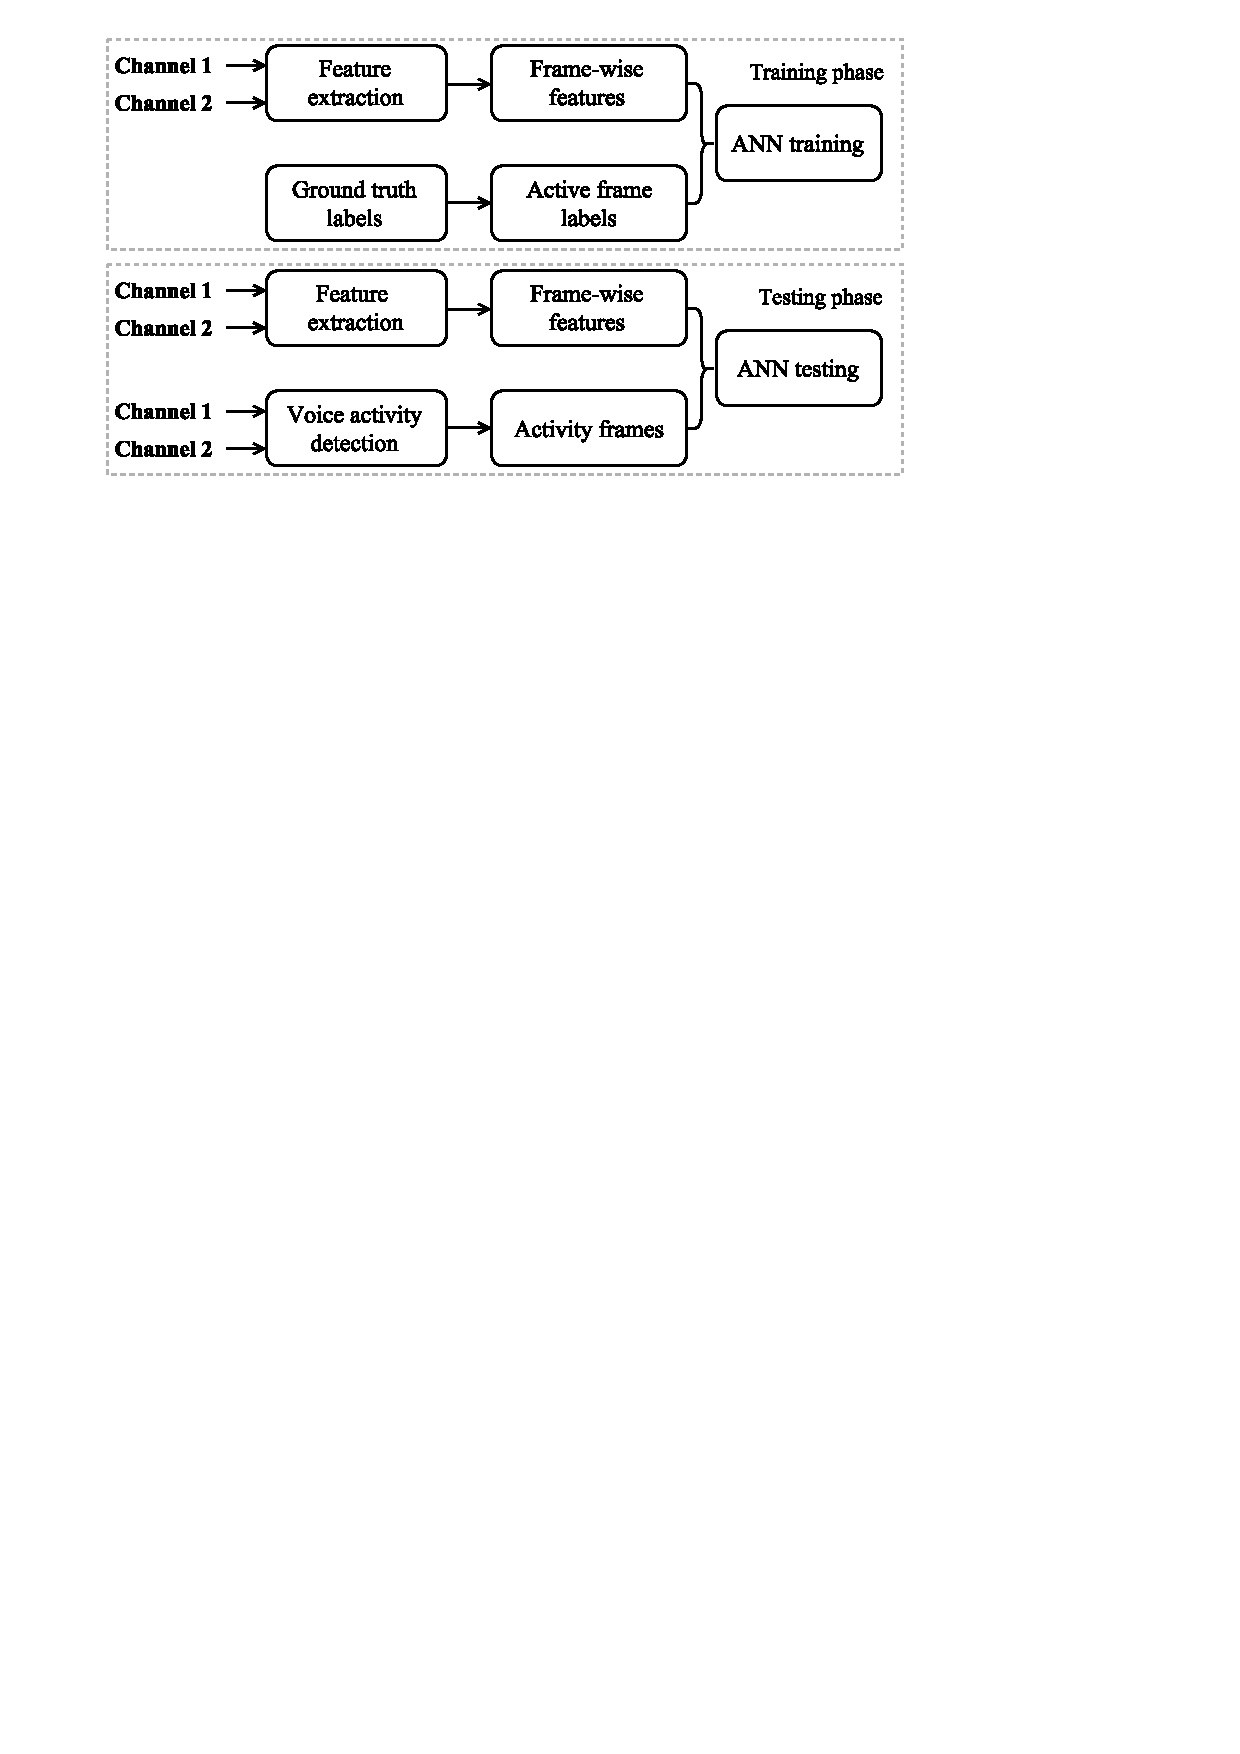
\includegraphics[width=0.47\textwidth]{figures/system_scheme.pdf}
	\caption{Block diagram of training and testing phases. At test time a VAD algorithm is used to determine onset and offset instants of the detected events.}
	\label{fig:system_scheme}
\end{figure}

\subsection{Feature representations}

In order to perform the SED task with ANNs, a set of one or more audio representations is typically extracted from the raw audio signal, that is the \emph{feature set}. Aiming to evaluate the impact of binaural information on the classification performance, we will, in the first instance, distinguish the proposed sets between monaural and binaural feature sets. We highlight that, for all the extracted feature sets, a frame-wise short-time Fourier transform (STFT) is firstly applied to the audio signal on frame windows of 40 ms with 50\% overlap. Moreover, all feature extraction processes described hereafter have been performed with openSMILE~\cite{eyben2013recent}, a license-free software package developed by the Technical University of Munich.

The first monaural set is known as log-mel spectrogram. In this case a down-mixing of the two audio channels is required before calculating the STFT coefficients. After the STFT coefficients are extracted, we apply a mel conversion of the frequency scale with a 26-bands mel-scale filter bank and compute the logarithm of all the energies so obtained. To complete the set, we also extract the first order delta coefficients operating on a context window of 10 frames. Given the log-mel coefficients and their respective deltas, this first set is composed of 52 coefficients for each frame.

The second monaural set is composed of another set of widely used features, that is mel-frequency cepstral coefficients (MFCCs). Starting from the same STFT coefficients previously obtained, we now compute the log-mel spectrogram with a 40-bands mel-scale filter bank. Then, we apply a 20-points discrete cosine transform (DCT) to each energy vector and, after excluding the 0\textsuperscript{th} order coefficient, we obtain a feature vector of 20 MFCCs. In order to complete the set, we also calculate the first and second order delta coefficients, therefore obtaining a 60-coefficients feature vector.

For the two binaural sets we decided to extract the log-mel (or the MFCC) features not only from the average of the two channels, but also from their difference and the two separate channels; this gives us a total of four channels. We decided to do so because, for example, if an important event is predominant in only one of the two channels, averaging them could lower the signal-to-noise ratio, thus increasing the system failure probability. For the first binaural set we extract the log-mel coefficients as for the first monaural set, but, given the presence of four channels, we now have a total of 108 coefficients for each frame. In order to avoid an excessive feature vector dimension, in this set we decide to avoid using the first and second order delta coefficients. Similarly, the second binaural set is obtained by extracting 20 MFCCs for each channel; since again we avoid using the delta coefficients, this leads us to a total of 80 coefficients for each frame. 

\subsection{Neural networks}

In this work two different ANNs architectures are tested for the SED problem, \emph{i.e.,}\ MLPs and RNNs. Asides from single layer perceptrons, MLPs can be considered to be the most simple (yet very effective) form of ANN. A MLP is composed of an ensemble of many nonlinear computational units (called neurons) organized in a layered structures. Thanks to the full connectedness of neurons between two sequent layers, each of them is likely trained to recognize a particular pattern occurring in a specific input position, therefore making the MLP able to build high level feature representations in deeper layers. 

RNNs, on the other hand, are a particular neural architecture designed to make use of the information obtained from prior network states, therefore giving the network the capability to ``remember'' past context information. This feature is obtained by adding a set of recursive connections going from and to each hidden neuron. Due this characteristic, the output is now computed only after a batch of input frames are forwarded into the network so that the final decision will rely on the correlation between different adjacent frames.

The first layer of all proposed ANNs consists of a set of nodes to which the audio representation (taken on a frame scale) is applied, with the number of nodes varying from 52 to 108, depending on the chosen feature representation. The input is then propagated to the following three hidden layers, composed of 512 tanh neurons each for MLPs and 54 rectifier neurons for RNNs.  Finally, the last layer of our networks is designed to output the class associated by the network with the given input. To do so, this layer is composed of a number of softmax neurons equal to the number of possible classes, \emph{i.e.,} 11 if we are dealing with a ``home'' scenario, and 7 in case of a ``residential area'' (see Tab.~\ref{tab:classes}). We highlight that, in case of MLPs, we obtain one label for each frame, whereas RNNs are able to output one label also for a batch of sequent frames.

The standard algorithm used for training the proposed MLPs is the backpropagation (BP) algorithm, whereas for RNNs the ``BP through time'' is used. After a first feed-forward phase, in which a batch of input is propagated through the networks, these algorithms exploit the derivative ``chain rule'' to back-propagate the error computed at the output layer and sequentially update all neuron weights~\cite{rojas2013neural}.

\subsection{Sound event detection and classification}

At test time we want the system to detect and correctly classify as many acoustic events as possible occurring in raw audio files of 30 seconds. Since no onset nor offset instants are given, we decide to use VAD algorithms in order to detect these instants. With this intent, two different VAD algorithms have been tested, \emph{i.e.,}\ AE, and Sohn's VAD. 

The AE approach makes use of two energy thresholds in order to determine the starting and ending point of an event-active audio sequence, \emph{i.e.,}\ the ``mean plus variance'' (MPV) and the ``mean minus variance'' (MMV) thresholds. These thresholds are firstly calculated over all the training dataset and then used to extract information about events activity: whenever a frame's energy exceeds the MPV threshold an onset event is triggered, then the event detection remains positive until the energy content drops below the MMV threshold. 

Sohn's VAD~\cite{sohn1999statistical}, on the other hand, is a method based on a statistical modelling of the audio in the time-frequency domain, with the model parameters being estimated with a maximum likelihood (ML) method. With this technique, the decision regarding the event's activity is devolved to a comparison between the averaged log-likelihood ratio (containing the a-priori and a-posteriori signal-to-noise ratios) and a fixed threshold $\eta \in (0,1)$. 

Whenever an audio file is processed by one of the two VAD algorithms we are able to extract the starting and ending instants between which an audio event has (supposedly) occurred. Hence, we can feed the network with the feature representation of the corresponding frames and finally obtain the event classification. We remind that, in case of MLPs, we obtain one label for each frame, whereas RNNs are able to output only one label for the whole frame batch. Due to this, we need to average all MLP outputs so to obtain the event's acoustic label, while RNN's outputs will need no further processing.

\section{Experiments}
\label{sec:eval}

\subsection{Datasets and metrics}

The data we use during our experiments consist of two datasets provided for the third task (SED in real life audio) of the DCASE 2016 challenge~\cite{mesaros2016tut}. The former dataset, called \emph{development dataset}, was at first provided in order to make all challengers able to compare their development results, while the latter, the \emph{evaluation dataset}, was used for the final evaluation of the submitted systems, so its ground truth was made public only a few weeks after the end of the challenge. Both datasets contains recordings of 3-5 minutes divided into two different acoustic scenarios: ``home'' and ``residential area''. Specific classes for each scenario are reported in Table~\ref{tab:classes}. 

%\begin{table}
%\caption{Classes for the ``home'' and ``residential area'' scenarios provided for the SED in real life audio task of the DCASE 2016 challenge.}
%\label{tab:classes}
%\centering
%\begin{tabular}{l l | l l}\toprule
%\multicolumn{2}{c}{\emph{Home}} & \multicolumn{2}{c}{\emph{Residential area}}\\
%\midrule
%rustling & glass jingling & banging & wind blowing\\
%snapping & object impact & bird singing\\
%cupboard & people walking & car passing by\\
%cutlery & washing dishes & children shouting\\
%dishes & water tap running & people walking  \\
%drawer & & people speaking \\
%\bottomrule
%\end{tabular}
%\end{table}

\begin{table}
	\caption{Classes and their occurrences for the ``home'' and ``residential area'' scenarios for the SED in real life audio task of the DCASE 2016 challenge.}
	\label{tab:classes}
	\centering
	\begin{tabular}{l c l c}\toprule
		\emph{Home} & \emph{Occurrences} & \emph{Residential area} & \emph{Occurrences}\\
		\midrule
		rustling & 60 & banging & 23\\
		snapping & 57 & bird singing & 271\\
		cupboard & 40 & car passing by & 108\\
		cutlery & 76 & children shouting & 31\\
		dishes & 151 & people walking & 52 \\
		drawer & 51 & people speaking & 44\\
		glass jingling & 36 & wind blowing & 30\\
		object impact & 250\\
		people walking & 54\\
		washing dishes & 84\\
		water tap running & 47\\
		\bottomrule
	\end{tabular}
\end{table}

The development dataset consists of 10 recordings for the ``home'' scenario, and 12 for the ``residential area'', and for both a four-folds cross-validation data splitting is provided by the organizers of the challenge. While creating the cross-validation folds, the challenge organizers imposed the only condition that the test subset does not contain classes unavailable in training subset, therefore the class distribution between the test subsets is not assumed to be uniform.

The evaluation dataset contains 5 recordings for both the ``home'' and the ``residential area'' scenarios each. For this dataset no cross-validation is performed, so it is possible to train only one system with all the development dataset (including files previously meant for testing purpose) and then test it with the evaluation files.

Scores used to evaluate all systems are the well known F1 and error rate (ER) scores, which are used to evaluate the system over segments of one second. Following the notation introduced in~\cite{mesaros2016tut}, for the evaluation purpose an event can be a: true positive (TP), if both the system and the ground truth indicate it as active; a false positive (FP), if the system indicates it as active, but it is not present in the ground truth; a false negative (FN), if the system does not detect it, but it is active in the ground truth. With this notation it is possible to define the precision (P), the recall (R), and the F1 score of the system as:
\begin{equation}
\text{P}=\frac{\text{TP}}{\text{TP}+\text{FP}}, \quad \text{R}=\frac{\text{TP}}{\text{TP}+\text{FN}}, \quad \text{F1}=\frac{2 \cdot \text{P} \cdot \text{R}}{\text{TP}+\text{FN}}.
\end{equation}

Concerning the ER, we must divide all possible errors into three categories: substitutions (S), insertions (I), and deletions (D). A substitution occurs when the system correctly detects an event but gives it the wrong label; moreover, we consider insertions all those FPs which are not substitutions, whereas we call deletions all those FNs which are not substitutions. According to this notation we define the ER as:
\begin{equation}
\text{ER} = \frac{\sum_{k=1}^{K} \text{S}(k) + \sum_{k=1}^{K} \text{D}(k) + \sum_{k=1}^{K} \text{I}(k)}{\sum_{k=1}^{K} \text{N}(k)},
\end{equation}
where $\text{N}(k)$ is the number of active events in the ground truth, and $k$ is the segment's index. Finally we highlight that, in obtaining the final score for the development dataset, we average the four per-fold scores as described in~\cite{mesaros2016tut}.

\subsection{Experimental setup}

Concerning the network training, we initialize all weights according to a normal distribution with zero mean and 0.1 variance. We then train the networks following the adam~\cite{kingma2014adam} method for stochastic optimization, for which we keep the default hyper-parameter configuration.

In order to prevent overfitting, for each fold we check the network performance on the respective fold's test set after each training epoch. If no improvement on this set is encountered for 60 consecutive epochs, the training is forced to an early stop. By doing so we are able to fine-tune the network hyper-parameters and obtain the architectures proposed in Section~\ref{sec:prop_meth}. 

After this phase we perform experiments on the evaluation data, for which we use the whole development training and test sets as training and validation data respectively. Then, at test time, we evaluate the system on the secret challenge data.

\subsection{Development results}

As introduced in Section~\ref{sec:prop_meth}, during our experiments we tested and compared different neural architectures, VAD algorithms, and feature representations. In Table~\ref{tab:dev_results_sohn} we report the results obtained with Sohn's VAD for 16 different system configurations, whereas in Table~\ref{tab:dev_results_ae} the same classifier and feature configurations are analysed in conjunction with AE VAD.

Table~\ref{tab:dev_results_sohn} highlights that the use of binaural audio features always enhances the system's performance in terms of both F1 and ER scores. Moreover, we can also notice that MLPs generally perform better than RNNs, in particular according to F1 scores, where no RNN manages to achieve more than 34.4\% F1 score. Finally, we report that the best system's configuration featuring Sohn's VAD is a MLP trained with binaural MFCC features, with a VAD threshold equal to 0.70. This system manages to reach 0.88 ER and 39.8\% F1 score, both averaged on the four folds.

\begin{table}
	\caption{Comparison of Scores obtained on the development dataset using different Features, Classifiers and Sohn's VAD Thresholds ($\eta$). Scores are Averaged among the four Cross-Validation Folds.}
	\label{tab:dev_results_sohn}
	\centering
	\begin{tabular}{l c c c c}\toprule
		\emph{Features} & \emph{$\eta$} & \emph{Classifier} & \emph{ER} & \emph{F1} (\%)\\
		\midrule
		Monaural log-mel & 0.98 & MLP & 0.93 & 34.6\\
		Binaural log-mel & 0.98 & MLP & 0.89 & 38.6\\
		\midrule
		Monaural log-mel & 0.70 & MLP & 0.90 & 35.4\\
		Binaural log-mel & 0.70 & MLP & 0.89 & 39.4\\
		\midrule
		Monaural MFCC & 0.98 & MLP & 0.92 & 35.7\\
		Binaural MFCC & 0.98 & MLP & 0.88 & 39.6\\
		\midrule
		Monaural MFCC & 0.70 & MLP & 0.91 & 36.2\\
		\textbf{Binaural MFCC} & \textbf{0.70} & \textbf{MLP} & \textbf{0.88} & \textbf{39.8}\\
		\midrule
		Monaural log-mel & 0.98 & RNN & 0.91 & 29.6\\
		Binaural log-mel & 0.98 & RNN & 0.88 & 35.6\\
		\midrule
		Monaural log-mel & 0.70 & RNN & 0.95 & 28.2\\
		Binaural log-mel & 0.70 & RNN & 0.88 & 34.4\\
		\midrule
		Monaural MFCC & 0.98 & RNN & 0.98 & 30.5\\
		Binaural MFCC & 0.98 & RNN & 0.88 & 34.1\\
		\midrule
		Monaural MFCC & 0.70 & RNN & 0.91 & 31.2\\
		Binaural MFCC & 0.70 & RNN & 0.88 & 31.0\\
		\bottomrule
	\end{tabular}
\end{table}

Table~\ref{tab:dev_results_ae} mostly confirms what emerged from the analysis of the previous table. Also with adaptive evergy VAD, the use of binaural features always improves the classification accuracy, even if differences are now less marked, with the highest improvement in F1 scores being +2\%. Moreover, it is interesting to notice that the difference between MLPs and RNNs accuracies is now reduced, maybe highlighting that the difference between their classification power thins if a better VAD algorithm leads to a better event detection. The best performing system featuring AE VAD is again a MLP which, with binaural log-mel features, manages to reach 0.78 ER and 43.1\% F1 scores, averaged on the four folds as for the previous results.

\begin{table}
	\caption{Comparison of Scores obtained on the development dataset using different Features, Classifiers and AE VAD. Scores are Averaged among the four Cross-Validation Folds.}
	\label{tab:dev_results_ae}
	\centering
	\begin{tabular}{l c c c}\toprule
		\emph{Features} & \emph{Classifier} & \emph{ER} & \emph{F1} (\%)\\
		\midrule
		Monaural log-mel & MLP & 0.78 & 41.2\\
		\textbf{Binaural log-mel} & \textbf{MLP} & \textbf{0.78} & \textbf{43.1}\\
		\midrule
		Monaural MFCC & MLP & 0.81 & 40.1\\
		Binaural MFCC & MLP & 0.82 & 42.1\\
		\midrule
		Monaural log-mel & RNN & 0.85 & 41.2\\
		Binaural log-mel & RNN & 0.82 & 43.1\\
		\midrule
		Monaural MFCC & RNN & 0.92 & 40.7\\
		Binaural MFCC & RNN & 0.89 & 41.0\\
		\bottomrule
	\end{tabular}
\end{table}

\subsection{Evaluation results}

\begin{table}
	\caption{Comparison of Scores obtained on the Evaluation Dataset using different Features, Classifiers and VAD Algorithms.}
	\label{tab:eval_results}
	\centering
	\begin{tabular}{l c c c c}\toprule
		\emph{Features} & \emph{VAD} & \emph{Classifier} & \emph{ER} & \emph{F1} (\%)\\
		\midrule
		Monaural log-mel & Sohn ($\eta=0.70$) & MLP & 0.80 & 40.2\\
		Binaural log-mel & Sohn ($\eta=0.70$) & MLP & 0.78 & 46.5\\
		\midrule
		Monaural MFCC & AE & MLP & 0.79 & 45.1\\
		\textbf{Binaural MFCC} & \textbf{AE} & \textbf{MLP} & \textbf{0.78} & \textbf{48.1}\\
		\midrule
		Monaural MFCC & AE & RNN & 0.82 & 41.0\\
		\bottomrule
	\end{tabular}
\end{table}

\begin{table}
	\caption{Comparison Between the proposed System and the three (out of 17) best performing DCASE 2016 Systems proposed for SED in real life audio.}
	\label{tab:challenge_results}
	\centering
	\begin{tabular}{l c c c c}\toprule
		\emph{Features} & \emph{VAD} & \emph{Classifier} & \emph{ER} & \emph{F1} (\%)\\
		\midrule
		\textbf{Binaural log-mel} & \textbf{AE} & \textbf{MLP} & \textbf{0.79} & \textbf{48.1}\\
		\midrule
		Binaural mel energy & - & RNN~\cite{adavanne2016sound} & 0.81 & 47.8\\
		Binaural mel energy & - & GMM~\cite{mesaros2016tut} & 0.88 & 23.7\\
		Binaural mel energy + TDOA & - & RNN~\cite{adavanne2016sound} & 0.89 & 34.3\\
		\bottomrule
	\end{tabular}
\end{table}

In Table~\ref{tab:eval_results} we report the main results for the most promising system configurations tested on the evaluation dataset. As we can see, scores tend to be higher than the ones obtained on the development dataset, especially for MLPs, highlighting the benefit introduced by the addition in the training set of those files previously used for testing. The expansion of the training set can be viewed as the expansion of the ``knowledge'' from which the network can learn at training time, therefore, when this happens, it is expectable to reach a better generalization performance. This behaviour is confirmed, the best performing configuration manages to achieve a 0.79 ER and 48.1\% F1 scores, and it consists of a MLP classifier trained on binaural MFCC features.

Table~\ref{tab:challenge_results} compares our best system to the three best performing ones proposed for the third task of the DCASE 2016 challenge. The first and the third ranks were achieved by Adavanne \emph{et al.}, which made use of RNN-LSTM architectures trained on spatial and harmonic features~\cite{adavanne2016sound} extracted from the two binaural channels. On the other hand, the second best system is the baseline proposed in~\cite{mesaros2016tut}, based on a GMM modelling of each acoustic event, plus one for the absence of sound events, which was trained with the non-labelled frame's features (MFCCs and their delta/delta-deltas were used). As we can see from the table, the proposed system manages to improve the F1 score by 0.3\% while reducing the error rate by 0.02.

\section{Conclusions and future work}
\label{sec:conclusions}

In this paper we proposed and evaluated a system for SED in real life audio. We compared different audio features, extracted in both monaural and binaural configurations, with which we trained different neural network classifiers. Moreover, we tested two different VAD algorithms for detecting sound activities to be classified by the proposed networks at test time. The proposed best performing system achieves an improvement on the winner of the third task in the DCASE 2016 challenge, thus highlighting the competitiveness of the proposed approach. Finally, given the improvement carried by the use of binaural features, we believe that future work should address the development of a binaural algorithm using one or more networks for each channel and a decision function for a decision fusion stage.